\section{x86}

\subsection{MSVC}

\IFRU{Что получаем на ассемблере компилируя MSVC 2010:}
{What we got after compiling in MSVC 2010:}

\lstinputlisting{patterns/04_scanf/ex1_MSVC.asm}

\IFRU{Переменная \TT{x} является локальной.}{Variable \TT{x} is local.} 

\IFRU{По стандарту \CCpp она доступна только из этой же функции и ниоткуда более. 
Так получилось, что локальные переменные располагаются в стеке. 
Может быть, можно было бы использовать и другие варианты, но в x86 это традиционно так.}
{\CCpp standard tell us it must be visible only in this function and not from any other point. 
Traditionally, local variables are placed in the stack. 
Probably, there could be other ways, but in x86 it is so.}

\index{x86!\Instructions!PUSH}
\IFRU{Следующая после пролога инструкция \TT{PUSH ECX} не ставит своей целью сохранить 
значение регистра \ECX. 
(Заметьте отсутствие соответствующей инструкции \TT{POP ECX} в конце функции)}
{Next instruction after function prologue, \TT{PUSH ECX}, has not a goal to save \ECX state 
(notice absence of corresponding \TT{POP ECX} at the function end).}

\IFRU{Она на самом деле выделяет в стеке 4 байта для хранения \TT{x} в будущем.} 
{In fact, this instruction just allocates 4 bytes on the stack for \TT{x} variable storage.} 

\label{stack_frame}
\index{\Stack!\IFRU{Стековый фрейм}{Stack frame}}
\index{x86!\Registers!EBP}
\IFRU{Доступ к \TT{x} будет осуществляться при помощи объявленного макроса \TT{\_x\$} 
(он равен -4) и регистра \EBP указывающего на текущий фрейм.}
{\TT{x} will be accessed with the assistance of the \TT{\_x\$} macro 
(it equals to -4) and the \EBP register pointing to current frame.}

\IFRU{Вообще, во все время исполнения функции, \EBP указывает на текущий \glslink{stack frame}{фрейм} и через \TT{EBP+смещение}
можно иметь доступ как к локальным переменным функции, так и аргументам функции.} 
{Over a span of function execution, \EBP is pointing to current \gls{stack frame} and it is possible 
to have an access to local variables and function arguments via \TT{EBP+offset}.}

\index{x86!\Registers!ESP}
\IFRU
{Можно было бы использовать \ESP, но он во время исполнения функции постоянно меняется. 
Так что можно сказать, что \EBP это \IT{замороженное состояние} \ESP на момент начала исполнения функции.}
{It is also possible to use \ESP, but it is often changing and not very convenient.
So it can be said, the value of the \EBP is \IT{frozen state} of the value of the \ESP at the moment of function execution start.}

\IFRU{Разметка типичного стекового \glslink{stack frame}{фрейма} в 32-битной среде}
{A very typical \gls{stack frame} layout in 32-bit environment is}:

\begin{center}
\begin{tabular}{ | l | l | }
\hline
\dots & \dots \\
\hline
EBP-8 & \IFRU{локальная переменная}{local variable} \#2, \MarkedInIDAAs{} \TT{var\_8} \\
\hline
EBP-4 & \IFRU{локальная переменная}{local variable} \#1, \MarkedInIDAAs{} \TT{var\_4} \\
\hline
EBP & \IFRU{сохраненное значение}{saved value of} \EBP \\
\hline
EBP+4 & \IFRU{адрес возврата}{return address} \\
\hline
EBP+8 & \argument \#1, \MarkedInIDAAs{} \TT{arg\_0} \\
\hline
EBP+0xC & \argument \#2, \MarkedInIDAAs{} \TT{arg\_4} \\
\hline
EBP+0x10 & \argument \#3, \MarkedInIDAAs{} \TT{arg\_8} \\
\hline
\dots & \dots \\
\hline
\end{tabular}
\end{center}

\IFRU
{У функции \scanf в нашем примере два аргумента.}{Function \scanf in our example has two arguments.}

\IFRU
{Первый ~--- указатель на строку содержащую \TT{``\%d''} и второй ~--- адрес переменной \TT{x}.} 
{First is pointer to the string containing \TT{``\%d''} and second~---address of variable \TT{x}.} 

\index{x86!\Instructions!LEA}
\IFRU{Вначале адрес \TT{x} помещается в регистр \EAX при помощи инструкции \TT{lea eax, DWORD PTR \_x\$[ebp]}.}
{First of all, address of the \TT{x} variable is placed into the \EAX register by \TT{lea eax, DWORD PTR \_x\$[ebp]} instruction}

\IFRU{Инструкция \LEA означает \IT{load effective address}, но со временем она изменила свою функцию}
{\LEA meaning \IT{load effective address} but over a time it changed its primary application}
~(\ref{sec:LEA}).

\IFRU{Можно сказать, что в данном случае \LEA просто помещает в \EAX результат суммы значения в регистре 
\EBP и макроса \TT{\_x\$}.}
{It can be said, \LEA here just stores sum of the value in the \EBP register and \TT{\_x\$} macro to the \EAX register.}

\IFRU{Это тоже что и}{It is the same as} \TT{lea eax, [ebp-4]}.

\IFRU{Итак, от значения \EBP отнимается $4$ и помещается в \EAX.
Далее значение \EAX заталкивается в стек и вызывается \scanf.}
{So, $4$ subtracting from value in the \EBP register and result is placed to the \EAX register.
And then value in the \EAX register is pushing into stack and \scanf is called.}

\IFRU{После этого вызывается \printf. Первый аргумент вызова которого, строка:} 
{After that, \printf is called. First argument is pointer to string:} \TT{``You entered \%d...\textbackslash{}n''}.

\IFRU{Второй аргумент: \TT{mov ecx, [ebp-4]}, эта инструкция помещает в \ECX не адрес переменной \TT{x}, 
а его значение, что там сейчас находится.}
{Second argument is prepared as: \TT{mov ecx, [ebp-4]},
this instruction places to the \ECX not address of the \TT{x} variable, but its contents.}

\IFRU{Далее значение \ECX заталкивается в стек и вызывается последний \printf.}
{After, value in the \ECX is placed on the stack and the last \printf called.}

\subsection{MSVC + \olly}
\index{\olly}

\IFRU{Попробуем этот же пример в}{Let's try this example in} \olly.
\IFRU{Загружаем, нажимаем F8 (\stepover) до тех пор, пока не окажемся в своем исполняемом файле,
а не в}{Let's load, press F8 (\stepover) until we get into our executable file
instead of} \TT{ntdll.dll}.
\IFRU{Скроллим вверх, до тех пока не найдем \main}{Scroll up until \main appears}.
\IFRU{Кликаем на первой инструкции}{Let's click on the first instruction} (\TT{PUSH EBP}), 
\IFRU{нажимаем}{press} F2, \IFRU{затем}{then} F9 (Run) \IFRU{и брякпойнт срабатывает
на начале \main}{and breakpoint triggers on the \main begin}.

\IFRU{Трассируем до того места, где готовится адрес переменной $x$}
{Let's trace to the place where the address of $x$ variable is prepared}:
\figname \ref{fig:scanf_ex1_olly_1}.

\IFRU{На \EAX в окне регистров можно нажать правой кнопкой и далее}
{It is possible to right-click on \EAX in registers window and then} ``Follow in stack''.
\IFRU{Этот адрес покажется в окне стека}{This address will appear in stack window}.
\IFRU{Смотрите, это переменная в локальном стеке}{Look, this is a variable in the local stack}.
\IFRU{Я нарисовал там красную стрелку}{I drawed a red arrow there}.
\IFRU{И там сейчас какой-то мусор}{And there are some garbage} (\TT{0x77D478}).
\IFRU{Адрес этого элемента стека сейчас, при помощи \PUSH, запишется в этот же стек, рядом}
{Now address of the stack element, with the help of \PUSH, will be written to the same stack, nearly}.
\IFRU{Трассируем при помощи F8 вплоть до конца исполнения \scanf}{Let's trace by F8 until \scanf 
execution finished}.
\IFRU{А пока \scanf исполняется, в консольном окне, вводим, например, 123}
{During the moment of \scanf execution, we enter, for example, 123, in the console window}:

\begin{figure}[H]
\centering
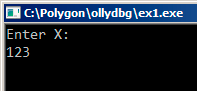
\includegraphics[scale=0.66]{patterns/04_scanf/ex1_olly_2.png}
\caption{\IFRU{Вывод в консоль}{Console output}}
\label{fig:scanf_ex1_olly_2}
\end{figure}

\RU{Вот тут }\scanf \IFRU{отработал}{executed here}: \figname \ref{fig:scanf_ex1_olly_3}. 
\scanf \IFRU{вернул}{returns} $1$ \InENRU \EAX, \IFRU{что означает, что он успешно прочитал одно 
значение}{which means, it have read one value successfully}.
\IFRU{В наблюдаемом нами элементе стека теперь}{The element of 
stack of our attention now contain} \TT{0x7B} (123).

\IFRU{Чуть позже, это значение копируется из стека в регистр \ECX и передается в \printf}
{Further, this value is copied from the stack to the \ECX register and passed into \printf}:
\figname \ref{fig:scanf_ex1_olly_4}.

\begin{figure}[H]
\centering
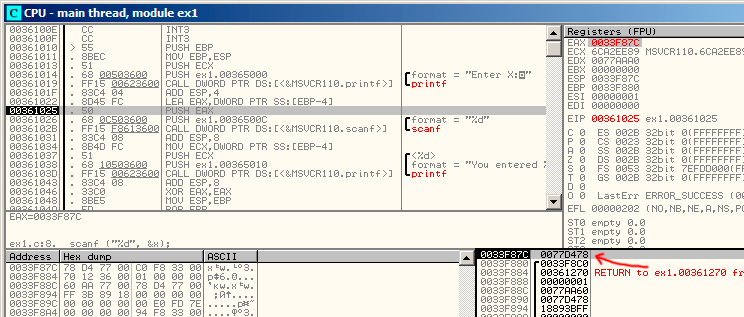
\includegraphics[scale=0.66]{patterns/04_scanf/ex1_olly_1.png}
\caption{\olly: \IFRU{вычисляется адрес локальной переменной}{address of the local variable is computed}}
\label{fig:scanf_ex1_olly_1}
\end{figure}

\begin{figure}[H]
\centering
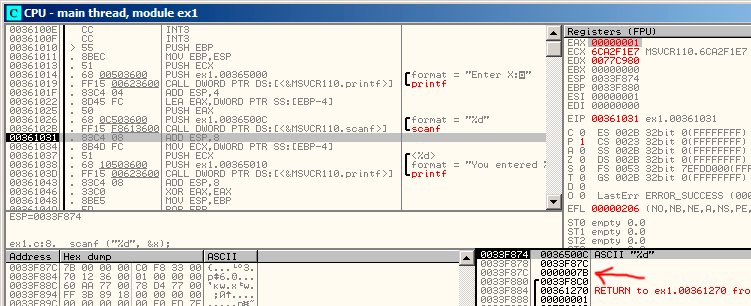
\includegraphics[scale=0.66]{patterns/04_scanf/ex1_olly_3.png}
\caption{\olly: \scanf \IFRU{исполнилась}{executed}}
\label{fig:scanf_ex1_olly_3}
\end{figure}

\begin{figure}[H]
\centering
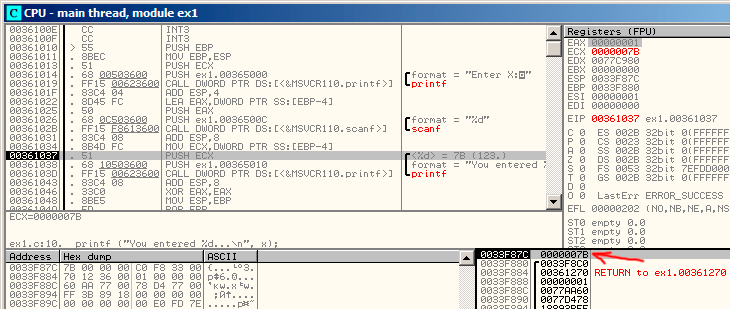
\includegraphics[scale=0.66]{patterns/04_scanf/ex1_olly_4.png}
\caption{\olly: \IFRU{готовим значение для передачи в}{preparing the value for passing into} \printf}
\label{fig:scanf_ex1_olly_4}
\end{figure}

\subsection{GCC}

\IFRU{Попробуем тоже самое скомпилировать в Linux при помощи GCC 4.4.1:}
{Let's try to compile this code in GCC 4.4.1 under Linux:}

\lstinputlisting{patterns/04_scanf/ex1_GCC.asm}

\index{puts() \IFRU{вместо}{instead of} printf()}
\IFRU{GCC заменил первый вызов \printf на \puts, почему это было сделано, 
уже было описано раннее~(\ref{puts}).}
{GCC replaced first the \printf call to the \puts, it was already described~(\ref{puts})
why it was done.}

% TODO: rewrite
%\IFRU
%{Почему \scanf переименовали в \TT{\_\_\_isoc99\_scanf}, я честно говоря, пока не знаю.}
%{Why \scanf is renamed to \TT{\_\_\_isoc99\_scanf}, I do not know yet.}

\IFRU{Далее все как и прежде ~--- параметры заталкиваются через стек при помощи \MOV.}
{As before~---arguments are placed on the stack by \MOV instruction.}
